\documentclass[12pt]{article}
\usepackage[margin=1in,left=1.2in,includefoot]{geometry}
\usepackage{enumerate}
\usepackage{longtable}
\usepackage{forest}
\usepackage[normalem]{ulem}
\usepackage{amsmath}
\usepackage{algorithm}
\usepackage{algpseudocode}
\usepackage{listings}
\usepackage{graphicx}
\usepackage{float}
\usepackage{subfig}

\lstset{%
   breaklines=true
}

\forestset{
  nice nodes/.style={
  for tree={
  inner sep=1pt, s sep=12pt,
  fit=band,
},
},
default preamble=nice nodes,
}
\useforestlibrary{linguistics}
\forestapplylibrarydefaults{linguistics}

\begin{document}
    \begin{titlepage}
        \begin{center}
            \vspace*{.06\textheight}{\scshape\LARGE Birkbeck, University of London\par}\vspace{1.5cm} % University name
            \rule[0.5ex]{\linewidth}{2pt}\vspace*{-\baselineskip}\vspace*{3.2pt}
            \rule[0.5ex]{\linewidth}{1pt}\\[\baselineskip]
            %title of the report
            \huge{\bfseries Fundamentals of Computing\\Coursework 2}\\[4mm]
            \rule[0.5ex]{\linewidth}{1pt}\vspace*{-\baselineskip}\vspace{3.2pt}
            \rule[0.5ex]{\linewidth}{2pt}\\
            [2.5cm]
        
            \textsc{\Large Baran Buluttekin\\13153116}\\
            [1.5cm]
            \large \textit{ I have read and understood the sections of plagiarism in the College Policy on assessment offences and confirm that the work is my own, with the work of others clearly acknowledged. I give my permission to submit my report to the plagiarism testing database that the College is using and test it using plagiarism detection software, search engines or meta-searching software.}


        \end{center}
    \end{titlepage}

    \section*{Answers}
    \begin{itemize}
        \item Baran Buluttekin
        \item Summation of values = 171
        \item Line number = 72
        \item X = 1 its 5th word
        \item words = consisted developing application area with which computer scientist would necessarily familiar such chemical testing dealing
        \item four letter version = cons, deve, appl, area, with, whic, comp, scie, woul, nece, fami, such, chem, test, deal  
    \end{itemize}
    \begin{enumerate}
        \item Threaded binary tree:
        
        \begin{forest}
            [HEAD, name=HEAD, draw    
                [cons, name=cons   [appl, name=appl   [,.phantom]
                                [area, name=area 
                                    [,.phantom]
                                    [comp, name=comp
                                        [chem]{\draw[->,dotted] () to [out=east, in=south] (comp);
                                        \draw[->,dotted] () to [out=west, in=south] (area);} 
                                        [,.phantom]
                                    ]{\draw[->,dotted] () to [out=east, in=south] (cons);} 
                                ]{\draw[->,dotted] () to [out=west, in=west] (appl);} 
                        ]{\draw[->,dotted] () to [out=west, in=west] (HEAD);} 
                        [deve, name=deve   
                                [deal]{\draw[->,dotted] () to [out=east, in=south] (deve);
                                \draw[->,dotted] () to [out=west, in=south] (cons);} 
                                [with, name=with
                                    [whic, name=whic 
                                        [scie, name=scie 
                                            [nece, name=nece
                                                [fami]{\draw[->,dotted] () to [out=east, in=south] (nece);
                                                \draw[->,dotted] () to [out=west, in=south] (deve);}
                                                [,.phantom]
                                            ]{\draw[->,dotted] () to [out=south east, in=south] (scie);}
                                            [such, name=such
                                                [,.phantom]
                                                [test]{\draw[->, dotted] () to [out=south west,in=south] (such);
                                                \draw[->, dotted] () to [out=south east,in=east] (whic); }
                                            ]{\draw[->,dotted] () to [out=south west, in=south] (scie);}
                                        ]
                                        [,.phantom]
                                    ]{\draw[->,dotted] () to [out=east, in=south] (with);}
                                    [woul]{\draw[->,dotted] () to [out=east, in=east] (HEAD);
                                    \draw[->,dotted] () to [out=west, in=south] (with);}
                                ]
                        ]
                ]
                [,.phantom]
            ]{\draw[->,dotted] () to [out=south east, in=north east] (HEAD);}    
            \end{forest}
        \item \textit{Post-order} traversed: chem, comp, area, appl, deal, fami, nece, test, such, scie, whic, woul, with, deve, cons
        \item Traversed \textit{pre-order} with algorithm from p.16: cons, appl, area, comp, chem, deve, deal, with, whic, scie, nece, fami, such, test, woul
        
        For the stack below left most item represent the first item in and right most item is the last item get in to the stack. Words crossed out represent item that was in the stack but popped out.
        
        My $3^{th}$ node is appl,\\
        Nodes visited: cons, appl \\
        Stack: cons \\

        My $6^{th}$ node is whic,\\
        Nodes visited: cons, appl, area, comp, chem, deve, deal, with, whic\\
        Stack: \sout{cons}, \sout{appl}, \sout{area}, \sout{comp}, \sout{chem}, \sout{deve}, \sout{deal}, with \\

        My $9^{th}$ node is woul, \\
        Nodes visited: cons, appl, area, comp, chem, deve, deal, with, whic, scie, nece, fami, such, test, woul\\
        Stack: \sout{comp, appl, area, comp, chem, deve, deal, with, whic, scie, nece, fami, such, test}\\

        My $12^{th}$ node is such,\\
        Nodes visited: cons, appl, area, comp, chem, deve, deal, with, whic, scie, nece, fami, such\\
        Stack: \sout{cons}, \sout{appl}, \sout{area}, \sout{comp}. \sout{chem}, \sout{deve}, \sout{deal}, with, whic, \sout{scie}, \sout{nece}, \sout{fami}\\

        \item $1^{st}$ item is cons, when removed:
        \begin{center}
        \begin{forest}
            [deal
                [appl
                    [,.phantom]
                    [area
                        [,.phantom]
                        [comp
                            [chem]
                            [,.phantom]
                        ]
                    ]
                ]
                [deve
                    [,.phantom]
                    [with
                        [whic
                            [scie
                                [nece
                                    [fami]
                                    [,.phantom]
                                ]
                                [such
                                    [,.phantom]
                                    [test]
                                ]
                            ]
                            [,.phantom]
                        ]
                        [woul]
                    ]
                ]
            ]
        \end{forest}
    \end{center}

    $2^{nd}$ item is deve, when removed:
    
    \begin{center}
        \begin{forest}
            [deal
                [appl
                    [,.phantom]
                    [area
                        [,.phantom]
                        [comp
                            [chem]
                            [,.phantom]
                        ]
                    ]
                ]
                [fami
                    [,.phantom]
                    [with
                        [whic
                            [scie
                                [nece]
                                [such
                                    [,.phantom]
                                    [test]
                                ]
                            ]
                            [,.phantom]
                        ]
                        [woul]
                    ]
                ]
            ]
        \end{forest}
    \end{center}

    $3^{rd}$ item is appl, when removed:

    \begin{center}
        \begin{forest}
            [deal
                [area
                    [,.phantom]
                    [comp
                        [chem]
                        [,.phantom]
                    ]
                ]
                [fami
                    [,.phantom]
                    [with
                        [whic
                            [scie
                                [nece]
                                [such
                                    [,.phantom]
                                    [test]
                                ]
                            ]
                            [,.phantom]
                        ]
                        [woul]
                    ]
                ]
            ]
        \end{forest}
    \end{center}
    \item We will obtain 4 fallowing trees.
    
    $1^{st} tree:$
    \begin{center}
        \begin{forest}
            [cons
                [appl]
                [area]
                [comp
                    [chem]
                ]
            ]
        \end{forest}
    \end{center}

    $2^{nd} tree:$
    \begin{center}
        \begin{forest}
            [deve
                [deal]
            ]
        \end{forest}
    \end{center}

    $3^{rd} tree:$
    \begin{center}
    \begin{forest}
        [with
            [whic
                [scie
                    [nece
                        [fami]
                    ]
                ]
                [such]
                [test]
            ]
        ]
    \end{forest}
    \end{center}

    $4^{th} tree:$
    \begin{center}
        Node: woul
    \end{center}
    \clearpage
    
    \item Algorithm:

    \begin{lstlisting}[mathescape=true]
        void FindLinkedNode(DataValue k, Treenode ROOT)
        {
            P $\leftarrow$ ROOT;
            // Find the node N
            while (P$\uparrow$INFO $\neq$ k)
            {
                P $\leftarrow$ P$\uparrow$LLINK if (P$\uparrow$INFO > k) else P$\uparrow$RLINK;
            }
            if (P = nil)
                repot_not_found();
            else
            { // Find the head node by moving along nodes head node will have a pinter Q
                Q $\leftarrow$ P$\uparrow$SUCC;
                while (Q$\uparrow$INFO $\neq$ 9999)
                {
                    Q $\leftarrow$ Q$\uparrow$SUCC;
                }
                // Once found delete the head note to replace to new position
                if (Q$\uparrow$SUCC $\neq$ P)
                {
                    Back $\leftarrow$ Q$\uparrow$PRED;
                    Front $\leftarrow$ Q$\uparrow$SUCC;
                    Back$\uparrow$SUCC $\leftarrow$ Front;
                    Front$\uparrow$PRED $\leftarrow$ Back;
                    // Insert head node after node N
                    Prev $\leftarrow$ P$\uparrow$PRED;
                    Prev$\uparrow$SUCC $\leftarrow$ Q;
                    Q$\uparrow$PRED $\leftarrow$ Prev;
                    Q$\uparrow$SUCC $\leftarrow$ P;
                    P$\uparrow$PRED $\leftarrow$ Q;
                }
            }
        }
    \end{lstlisting}
    \clearpage

    \item B-tree examples
    
    \textbf{Strategy for data-pages: }
    \begin{enumerate}
        \item Odd number items will always be on the left-hand page.
        \item When merging a page, I will always merge with the left-hand page. Unless the page doesn't have a left page or merging with left-hand page cause overflowing data-page.
    \end{enumerate}

    m = 6 r = 6\\
    Inserting JAM:

    This item will be inserted to data page of [HIP, $\cdots$, MUD]. This data page have one more record space available, record can be added without any split.

    \begin{figure}[H] \label{fig:insertjam}
        \centering
        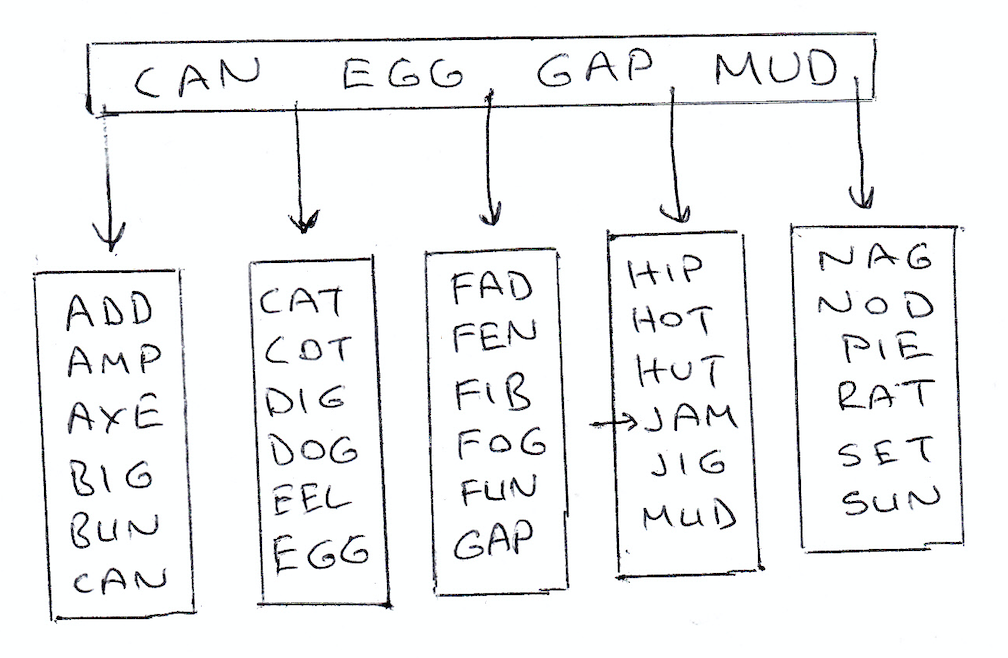
\includegraphics[width=\textwidth]{img/insertjam.png}
    \end{figure}

    Inserting OWL:

    This record should be inserted to data-page of [NAG, $\cdots$, SUN]. This page have already 6 item, adding this record will split the page. Final result will have max number of pointer page.

    \begin{figure}[H] \label{fig:insertowl}
        \centering
        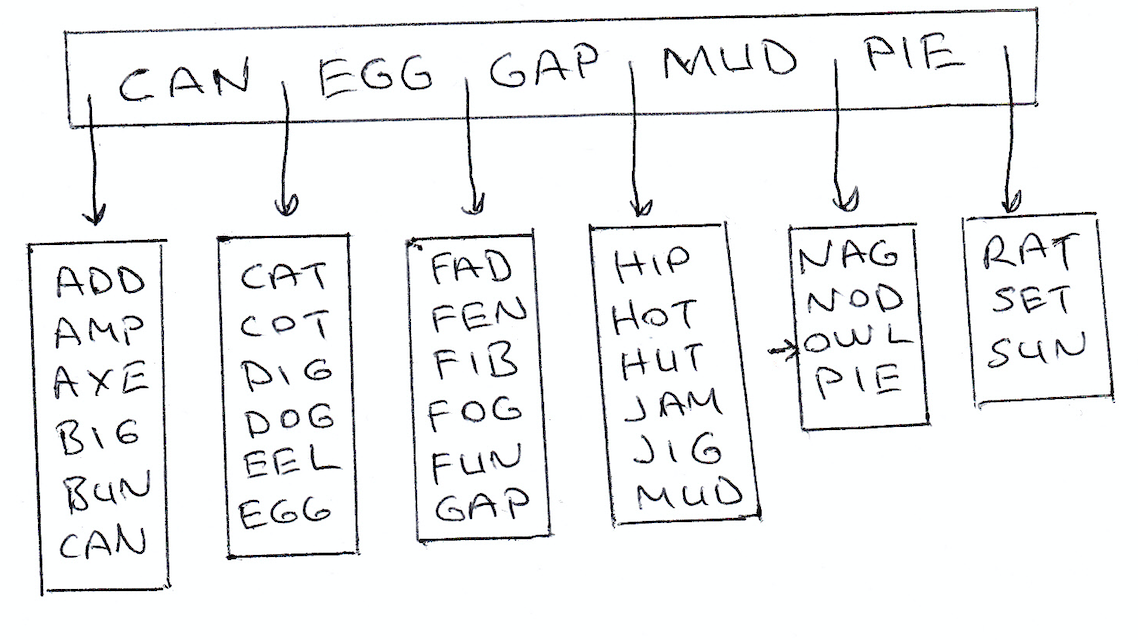
\includegraphics[width=\textwidth]{img/insertowl.png}
    \end{figure}

    Inserting NET:

    Does not cause split just inserted.

    \begin{figure}[H] \label{fig:insertnet}
        \centering
        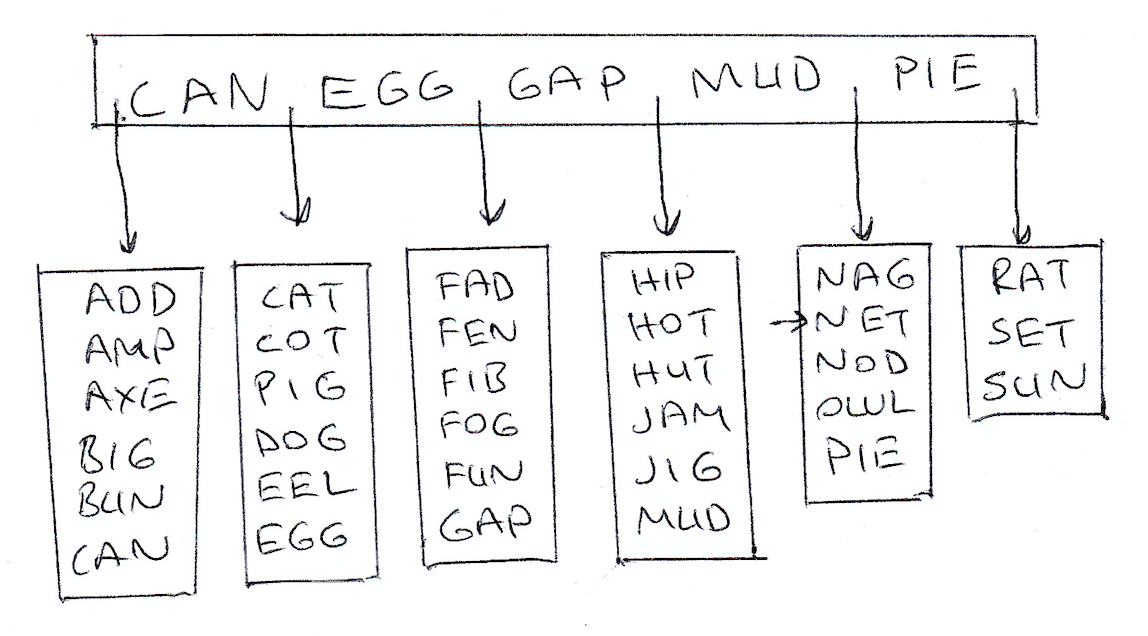
\includegraphics[width=\textwidth]{img/insertnet.png}
    \end{figure}

    Inserting OXO:

    Does not cause any split but the data-page it goes into have maximum number of data.

    \begin{figure}[H] \label{fig:insertoxo}
        \centering
        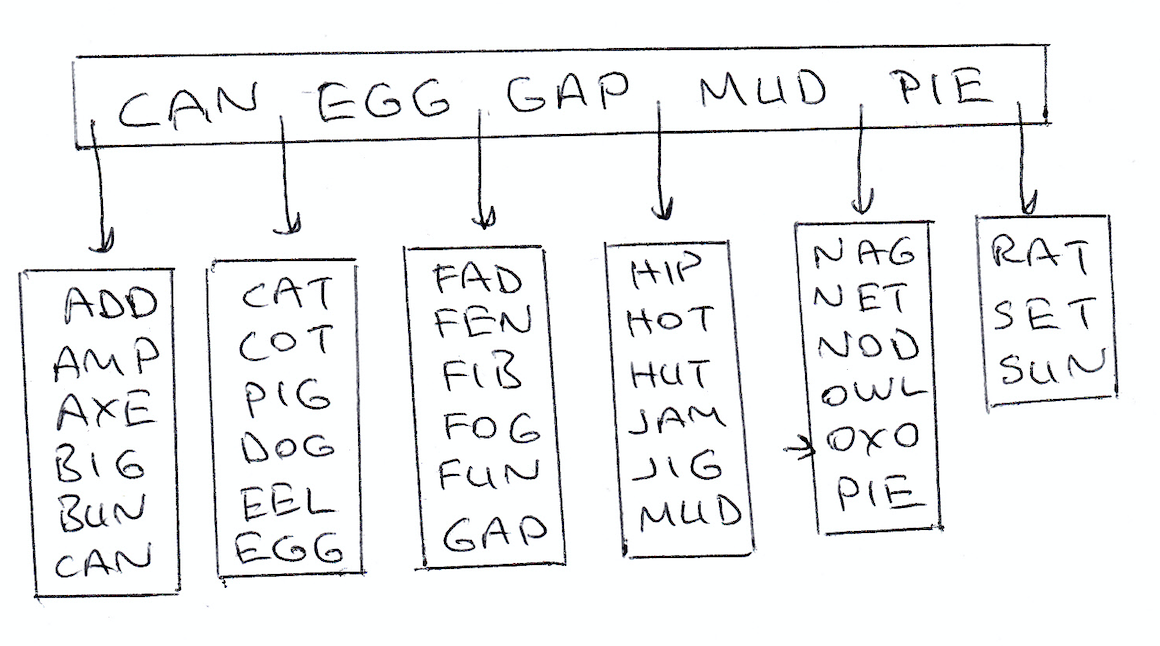
\includegraphics[width=\textwidth]{img/insertoxo.png}
    \end{figure}

    Inserting LOG:

    This will go to data-page [HIP, $\cdots$, MUD]. Result is a split data-page. Because the maximum number of pointer pages reached in this level the key we obtain will go to layer up.

    \begin{figure}[H] \label{fig:insertlog}
        \centering
        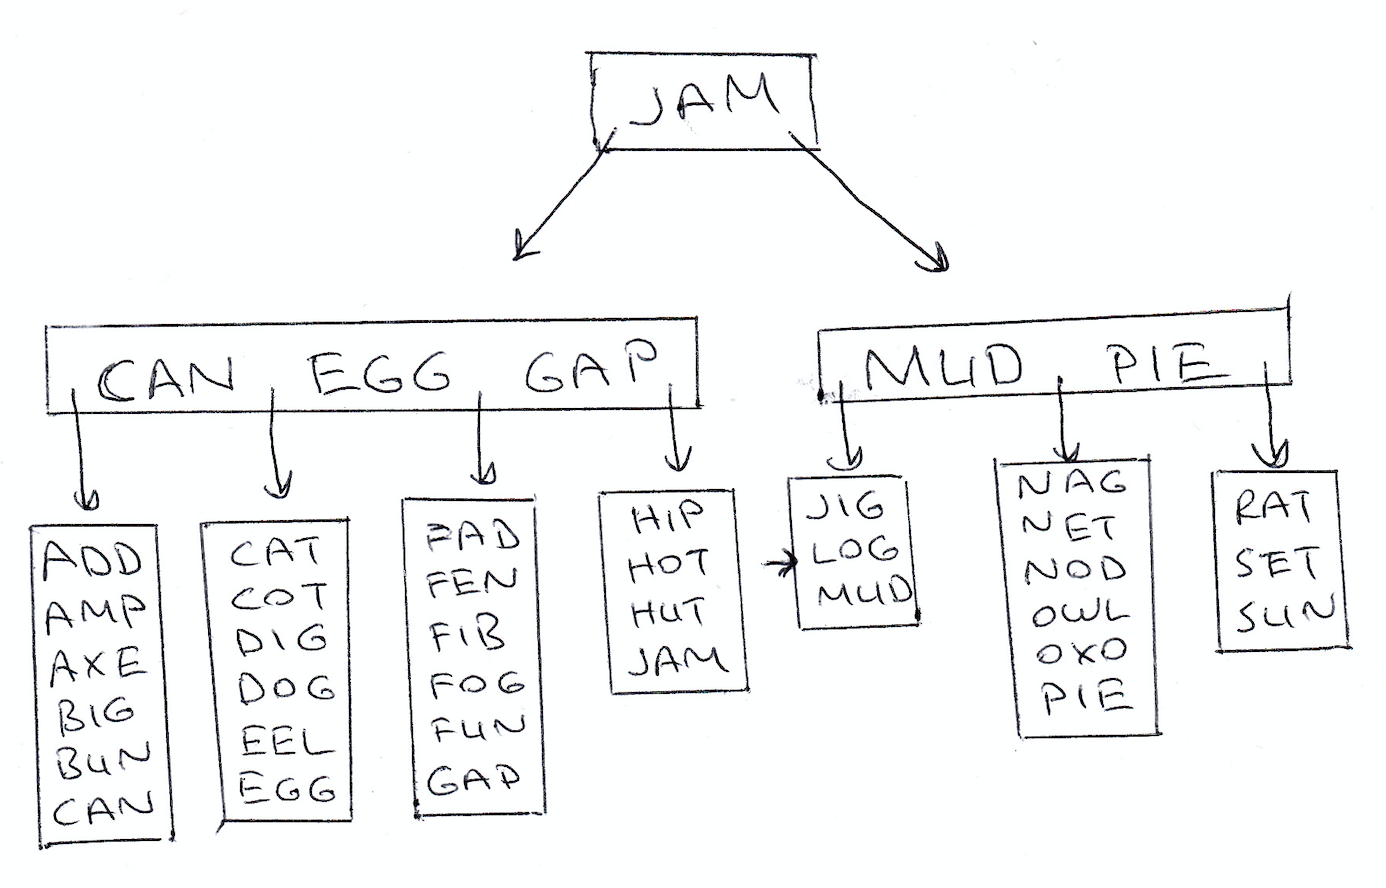
\includegraphics[width=\textwidth]{img/insertlog.png}
    \end{figure}

    \item Deletion 
    
    m = 5 and r = 4\\
    Deleting RIM:

    When RIM is deleted data-page it was occupying will have less than min number record and needs to be merged with another page. Because there is no left page in this pointer page I merged it with right data-page. and key SAG not in use can be removed. Removing that key will leave that pointer page less than minimum number of pointer pages and we ca merge it with left pointer page to avoid it. Top level key PIN no longer required and we can bring it to lover level to pointer-page.
    \begin{figure}[H] \label{fig:deleterim}
        \centering
        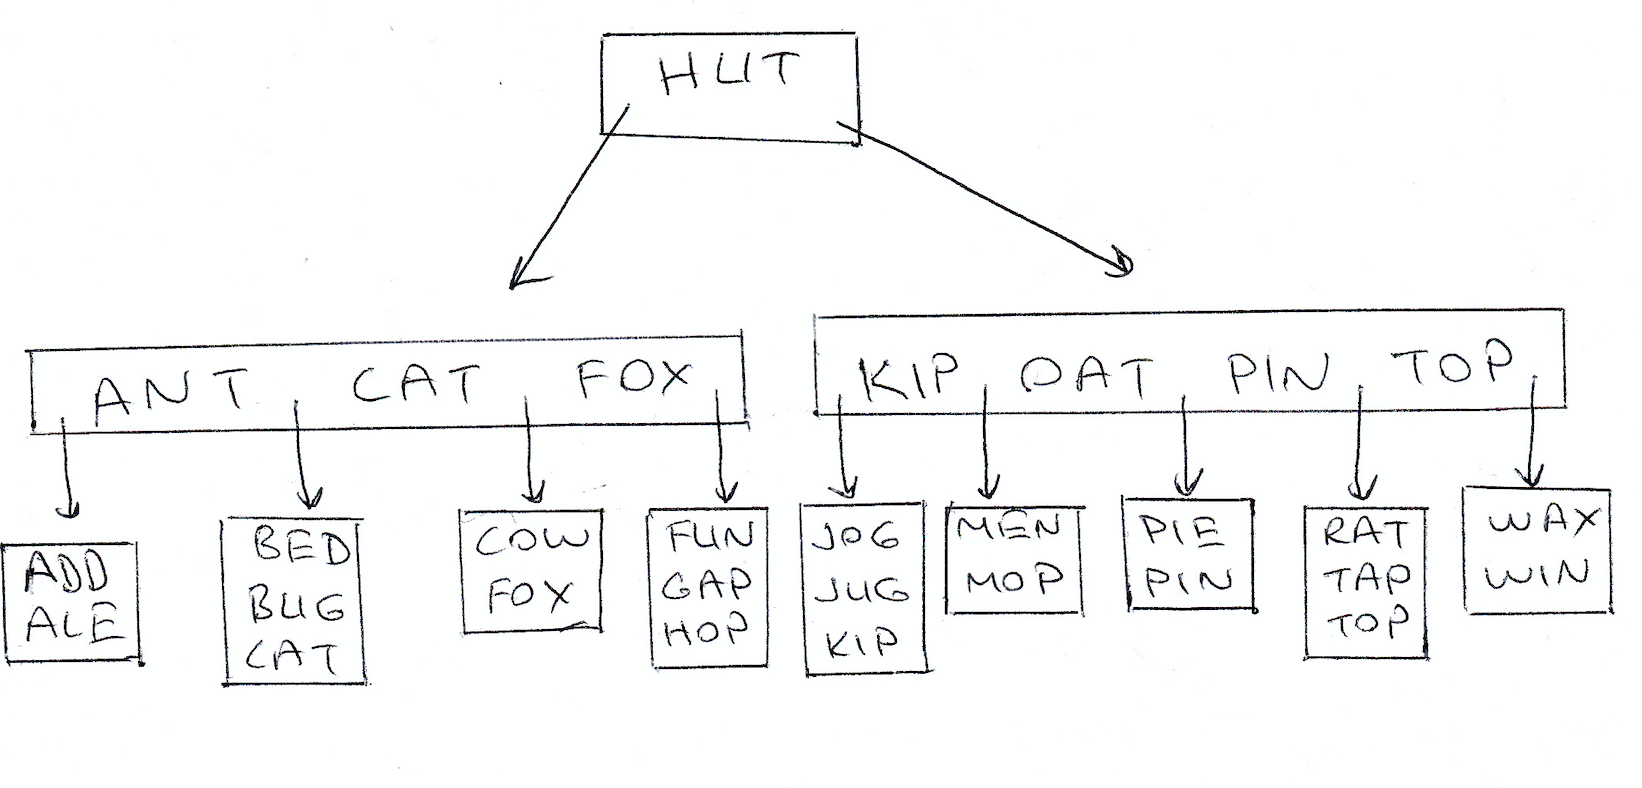
\includegraphics[width=\textwidth]{img/deleterim.png}
    \end{figure}

    Deleting ALE:

    When we delete ALE data-page it was in will have to merge. In this case there is no left page thats why I merged it with right page. It's pointer page no longer in use can deleted.
    \begin{figure}[H] \label{fig:deleteale}
        \centering
        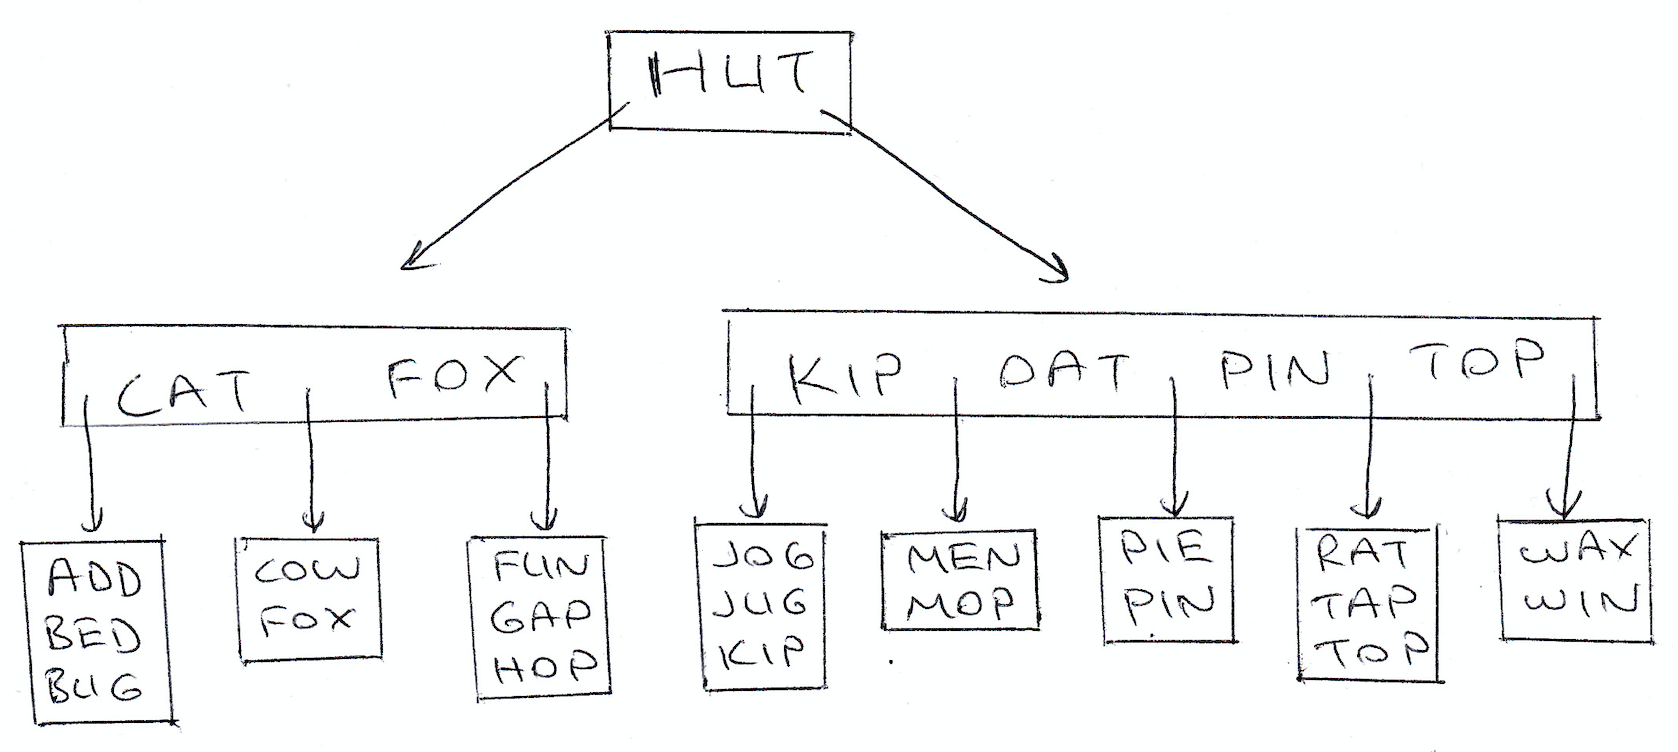
\includegraphics[width=\textwidth]{img/deleteale.png}
    \end{figure}

    Deleting COW:

    Deleting COW also require merging. When merged CAT key is not needed and can be deleted. After the key deleted this pointer page does not have enough data-page and have to be merged with next pointer-page. Upper level HUT is used in merging but the end result have more than maximum number of pointer-pages. I split the pointer pages by taking KIP key to upper level.
    \begin{figure}[H] \label{fig:deletecow}
        \centering
        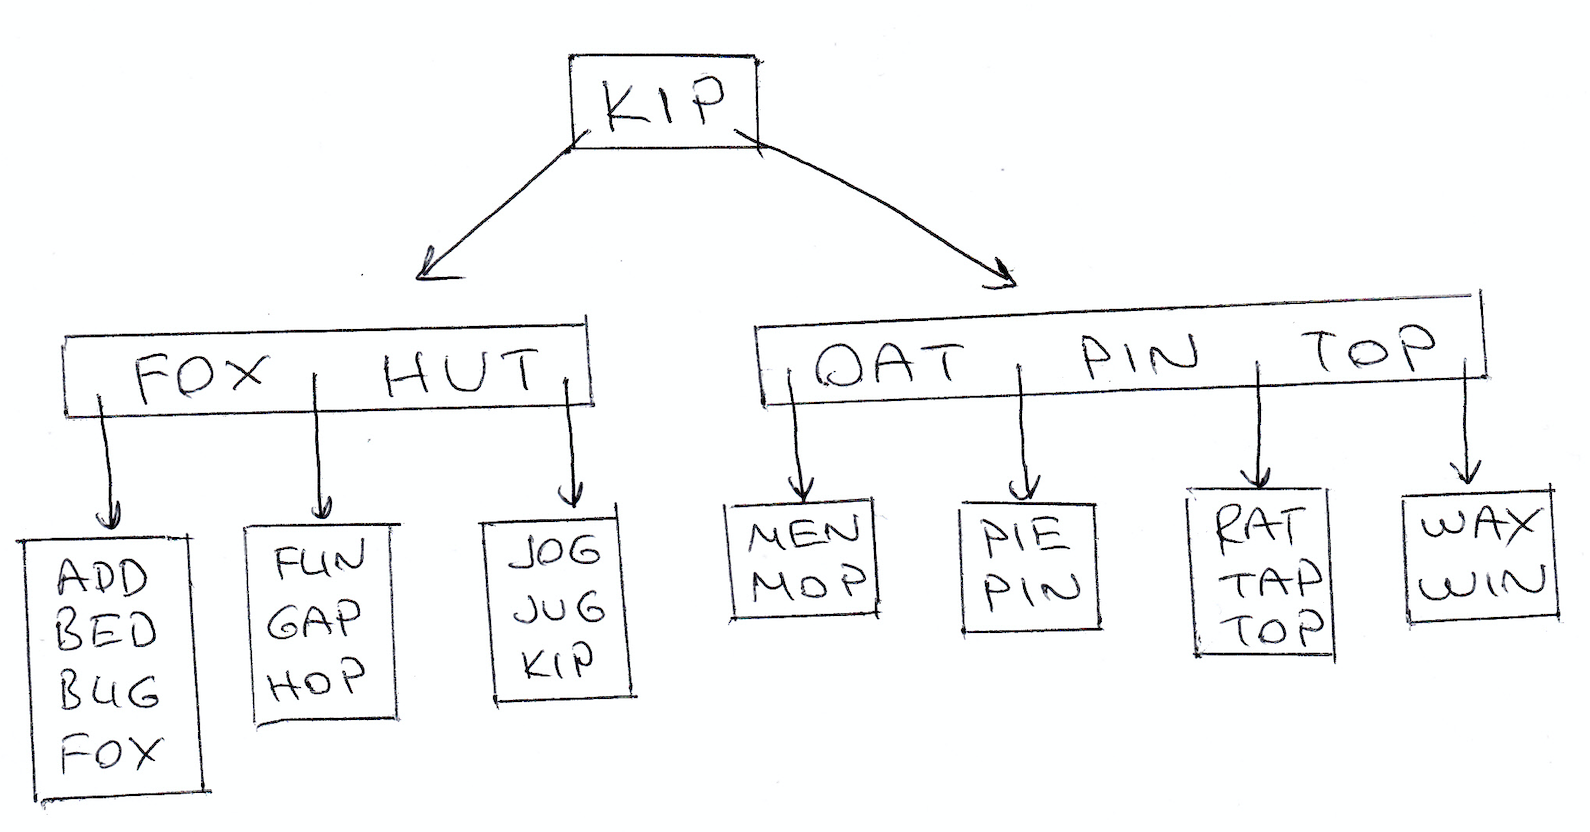
\includegraphics[width=\textwidth]{img/deletecow.png}
    \end{figure}

    \item Delete RAT:
    
    m = 5 and r = 4\\
    When the RAT is deleted data-page have to merge with left data-page and key PIN can be deleted. Result then have insufficient number of pointer pages. Have to be merged with left pointer page by bringing the top level key FOX down.
    \begin{figure}[H] \label{fig:deleterat}
        \centering
        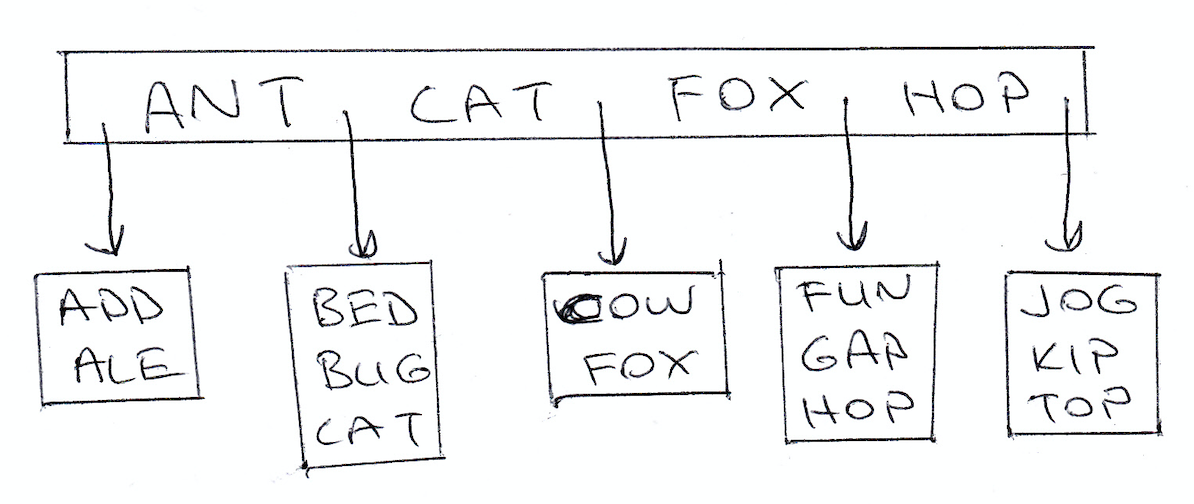
\includegraphics[width=\textwidth]{img/deleterat.png}
    \end{figure}

    \end{enumerate}

\end{document}